\documentclass{article}

\usepackage[final]{iai_neurips_2024}
\bibliographystyle{unsrtnat}
\newtheorem{definition}{Definition}
\newtheorem{proposition}{Proposition}
\usepackage{amsmath}
\usepackage{algorithm}
\newcommand{\isometrypursuit}{{\sc IsometryPursuit}}
\usepackage[font=small]{caption}
\captionsetup[algorithm]{labelformat=empty}
% \usepackage{algpseudocode}
\usepackage{algorithmic}

\newcommand{\M}{\mathcal{M}}
\newcommand{\N}{\mathcal{N}}


\title{Isometry pursuit}

\author{%
  Samson Koelle \\
  Amazon Web Services  \\
  Seattle, WA
  \And
  Marina Meila \\
  Department of Statistics\\
  University of Washington \\
  Seattle, WA \\
}

\begin{document}

\maketitle

\begin{abstract}
Isometry pursuit is a convex algorithm for identifying orthonormal column-submatrices of wide matrices.
It consists of a novel normalization method followed by multitask basis pursuit.
Applied to Jacobians of putative coordinate functions, it helps identity isometric embeddings from within interpretable dictionaries.
We provide theoretical and experimental results justifying this method.
It appears to be more accurate than greedy search and more efficient than brute force search.
\end{abstract}


\footnotetext[1]{Work conducted outside of Amazon.}

\section{Introduction}
\label{sec:introduction}

Many real-world problems may be abstracted as selecting a subset of the columns of a matrix representing stochastic observations or analytically exact data.
This paper focuses on a simple such problem that appears in interpretable learning and diversification.
Given a rank $D$ matrix $ X \in \mathbb R^{D \times P}$ with $P > D$, select a square submatrix $ X_{.\mathcal S}$ where subset $ S \subset P$ satisfies $| S| = D$ that is as orthonormal as possible.

This problem arises in interpretable learning specifically because while the coordinate functions of a given feature space may have no intrinsic meaning, it is sometimes possible to generate a dictionary of interpretable features which may be considered as potential parametrizing coordinates.
When this is the case, selection of candidate interpretable features as coordinates can take the above form.
While implementations vary across data and algorithmic domains, identification of such coordinates generally aids mechanistic understanding, generative control, and statistical efficiency.

This paper shows that an adapted version of the algorithm in \citet{Koelle2024-no} leads to a convex procedure that can improve upon greedy approaches such as those in \citet{5895106, NEURIPS2019_6a10bbd4, Kohli2021-lr, Jones2007-uc} for finding isometries.
The insight leading to isometry pursuit is that multitask basis pursuit applied to an appropriately normalized $ X$ selects orthonormal submatrices.
Given vectors in $\mathbb R^D$, the normalization log-symmetrizes length and favors those closer to unit length, while basis pursuit favors those which are orthogonal.
Our results formalize this intuition within a limited setting, and show the usefulness of isometry pursuit as a trimming procedure prior to brute force search for diversification and interpretable coordinate selection.
We also introduce a novel ground truth objective function to measure the success of our algorithm against, and discuss the reasonableness of this trimming procedure.

 \footnotetext[2]{Code is available at \url{https://github.com/sjkoelle/isometry-pursuit}.}
\section{Background}

In this section, we give background on the isometry and diversification problems, as well as the spectral and convex analysis that motivate our method.

\subsection{Problem}

Our goal is, given a matrix $ X \in \mathbb R^{D \times P}$, to select a subset $ S \subset [P]$ with $| S| = D$ such that $X_{.  S}$ is as orthonormal as possible in a computationally efficient way.
% To this end, we define a ground truth loss function that measures orthonormalness, and then introduce a surrogate loss function that convexifies the problem.

\subsection{Interpretability and isometry}

One motivating example is the selection of data representations from within sets of putative coordinates: the columns of a provided wide matrix.
This method applies to interpretability, for which parsimony is at a premium.
Interpretability arises through comparison of data with what is known to be important in the domain of the problem.
This knowledge often takes the form of a functional dictionary.
Evaluation of independence of dictionary features arises in numerous scenarios \citep{Chen2019-km, Koelle2022-ju, He2023-ch}.
The requirement that dictionary features be full rank has been called functional independence \citep{Koelle2022-ju} or feature decomposability \citep{templeton2024scaling}, with connection between dictionary rank and independence via the implicit function theorem.
Besides independence, the metric properties of such dictionary elements are of natural interest.
This is formalized through the notion of differential.

\begin{definition}
The \textbf{differential} of a smooth map $\phi:\mathcal M \to \mathcal N$ between $D$ dimensional manifolds $\M \subseteq \mathbb R^B$ and $\N \subseteq \mathbb R^P$ is a map in tangent bases $x_1 \dots x_{D}$ of $T_\xi \M$ and $y_1 \dots y_{D}$ of $T_{\phi(\xi)} \N$ consisting of entries
\begin{align}
\label{eq:diff}
    D\phi (\xi) = \begin{bmatrix}
    \frac{\partial \phi_1  }{\partial x_1}(\xi)  & \dots & \frac{\partial \phi_1 }{\partial x_D}(\xi)  \\
    \vdots & & \vdots \\
    \frac{\partial \phi_D }{\partial x_1}(\xi)  & \dots & \frac{\partial \phi_{D}  }{\partial x_{D}}(\xi) 
    \end{bmatrix}.
\end{align}
\end{definition}

It is not always necessary to explicitly estimate tangent spaces when applying this definition.
The most commonly encountered manifolds are vector spaces for which the tangent spaces are trivial.
This is the case for full-rank tabular data, for which isometry has a natural interpretation as a type of diversification, and often for the latent spaces of deep learning models.
In this case, $B = D$.

\begin{definition}
\label{def:isometric_at_a_point}
A map $\phi$ between $D$ dimensional submanifolds with inherited Euclidean metric $\mathcal M \subseteq R^{B}$ and $\mathcal N  \subseteq R^{P}$
$\phi$ is an \textbf{isometry at a point} $\xi \in \mathcal M$ if
\begin{align}
{D \phi (\xi)}^T D \phi (\xi) = I_D.
\end{align}
That is, $\phi$ is an isometry at $\xi$ if $D \phi (\xi)$ is orthonormal.
\end{definition}

The applications of pointwise isometry are themselves manifold.
Pointwise isometric embeddings faithfully preserve high-dimensional geometry.
For example, Local Tangent Space Alignment \citep{ZhangZ:04}, Multidimensional Scaling \citep{ChenBuja:localMDS09} and Isomap \citep{tenenbaum2000ggf} non-parametrically estimate embeddings that are as isometric as possible.
Another approach stitches together pointwise isometries selected from a dictionary to form global embeddings \citep{Kohli2021-lr}.
The method is particularly relevant since it constructs such isometries through greedy search, with putative dictionary features added one at a time.

That $D\phi$ is orthonormal has several equivalent formulations.
The one motivating our ground truth loss function comes from spectral analysis.
\begin{proposition}
\label{prop:orthonormal_spectrum}
The singular values $\sigma_1 \dots \sigma_D$ are equal to $1$ if and only if $U \in \mathbb{R}^{D \times D}$ is orthonormal.
\end{proposition}
On the other hand, the formulation that motivates our convex approach is that orthonormal matrices consist of $D$ coordinate features whose gradients are orthogonal and of unit length.
\begin{proposition}
\label{prop:orthonormal_basis}
The component vectors $u_1 \dots u_D \in \mathbb R^B$ form a orthonormal matrix if and only if, for all $d_1, d_2 \in [D], \langle u_{d_1}, u_{d_2} \rangle = \begin{cases}
1 \; d_1 = d_2 \\ 
0 \; d_1 \neq d_2 
\end{cases}$.
\end{proposition}

\subsection{Diversification}

Cosine
MMR definition.
Embeddings - sim is just projection

\subsection{Best subset selection}

Given a matrix $ X \in \mathbb R^{D \times P}$, we compare algorithmic paradigms for solving problems of the form
\begin{align}
\label{prog:ground_truth}
\arg \min_{ S \in \binom{[P]}{D}} l ( X_{. S})
\end{align}
where $\binom{[P]}{D} = \left\{ A \subseteq [P] : \left|A\right| = D \right\}$.
Brute force algorithms consider all possible solutions.
These algorithms are conceptually simple, but have the often prohibitive time complexity $O(C_lP^D)$ where $C_l$ is the cost of evaluating $l$.
Greedy algorithms consist of iteratively adding one element at a time to $ S$.
This algorithms have time complexity $O(C_lPD)$ and so are computationally more efficient than brute force algorithms, but can get stuck in local minima.
Formal definitions are given in Section \ref{sec:algorithms}.

Sometimes, it is possible to introduce an objective which convexifies problems of the above form.
Solutions
\begin{align}
\arg \min f(\beta) : Y  = X\beta 
\end{align}
to the overcomplete regression problem $Y = X \beta$ are a classic example \citep{Chen2001-hh}.
When $f(\beta) = \|\beta\|_0$, this problem is non-convex, and is thus suitable for greedy or brute algorithms, but when $f(\beta) =\|\beta\|_1$, the problem is convex, and may be solved efficiently via interior-point methods.
When the equality constraint is relaxed, Lagrangian duality may be used to reformulate as a so-called Lasso problem, which leads to an even richer set of optimization algorithms. % cite FISTA< glmnet, coordinate descent

The form of basis pursuit that we apply is inspired by the group basis pursuit approach in \citet{Koelle2022-ju}.
In group basis pursuit (which we call multitask basis pursuit when grouping is dependent only on the structure of matrix-valued response variable $y$) the objective function is $f(\beta) = \|\beta\|_{1,2} := \sum_{p=1}^P \|\beta_{p.}\|_2$  \citep{Yuan2006-bt, Obozinski2006-kq, Yeung2011-fg}.
This objective creates joint sparsity across entire rows $\beta_{p.}$ and was used in \citet{Koelle2022-ju} to select between sets of interpretable features.

\begin{frame}{Dictionary-based manifold learning}
\begin{algorithm}[H]
\caption{\tsalg(Dataset $\mathcal D$, dictionary $g$)}
\begin{algorithmic}[1]
\STATE Compute Jacobian $d g (n) \in \mathbb R^{P \times B} \; \forall  n \in [N]$
\STATE Normalize $\|d g^p \|_F = \sqrt{N} \; \forall  p \in [P]$
\STATE Estimate tangent basis $T_{\mathcal M}(n) \in \mathbb R^{D \times B} \; \forall  n \in [N]$
\STATE Project $d_\M g (n) = {T_{\mathcal M} (n)}^T d g (n) \; \forall  n \in [N]$
\STATE  $\hat \beta \gets \arg \min_{\beta \in \mathbb R^{N \times P \times D}} J_\lambda ( d_\M g ([N]),\beta)$ (Group Lasso)
\STATE {\bf Output} $S= \supp \hat  \beta$ 
\end{algorithmic}
\end{algorithm}
\begin{itemize}
\item $J_\lambda (X, \beta) =  \frac{1}{2}\sum_{n=1}^N \| I_D  - X_{n..} \beta_{n..}\|_F^2+\frac{\lambda}{\sqrt{DN}} \sum_{p=1}^P \|\beta_{.p.}\|_F. $
\item Optimize with FISTA
\item Locate region on regularization path with $|S| = D$ using binary search
\end{itemize}
\end{frame}


\begin{frame}{Estimating tangent spaces using local PCA}
\begin{columns}
\begin{column}{0.35\textwidth}
\begin{itemize}
    \item First, perform a nearest neighbor search around $\xi = \mathcal D(n) \in \mathcal M$
    \item Then, estimate $ T_{\mathcal M}(n) $ using the top singular vectors $[x^1, \dotsc x^D]$ of the centered neighbors
\end{itemize}
\end{column}
\begin{column}{0.6\textwidth}
\begin{figure}
    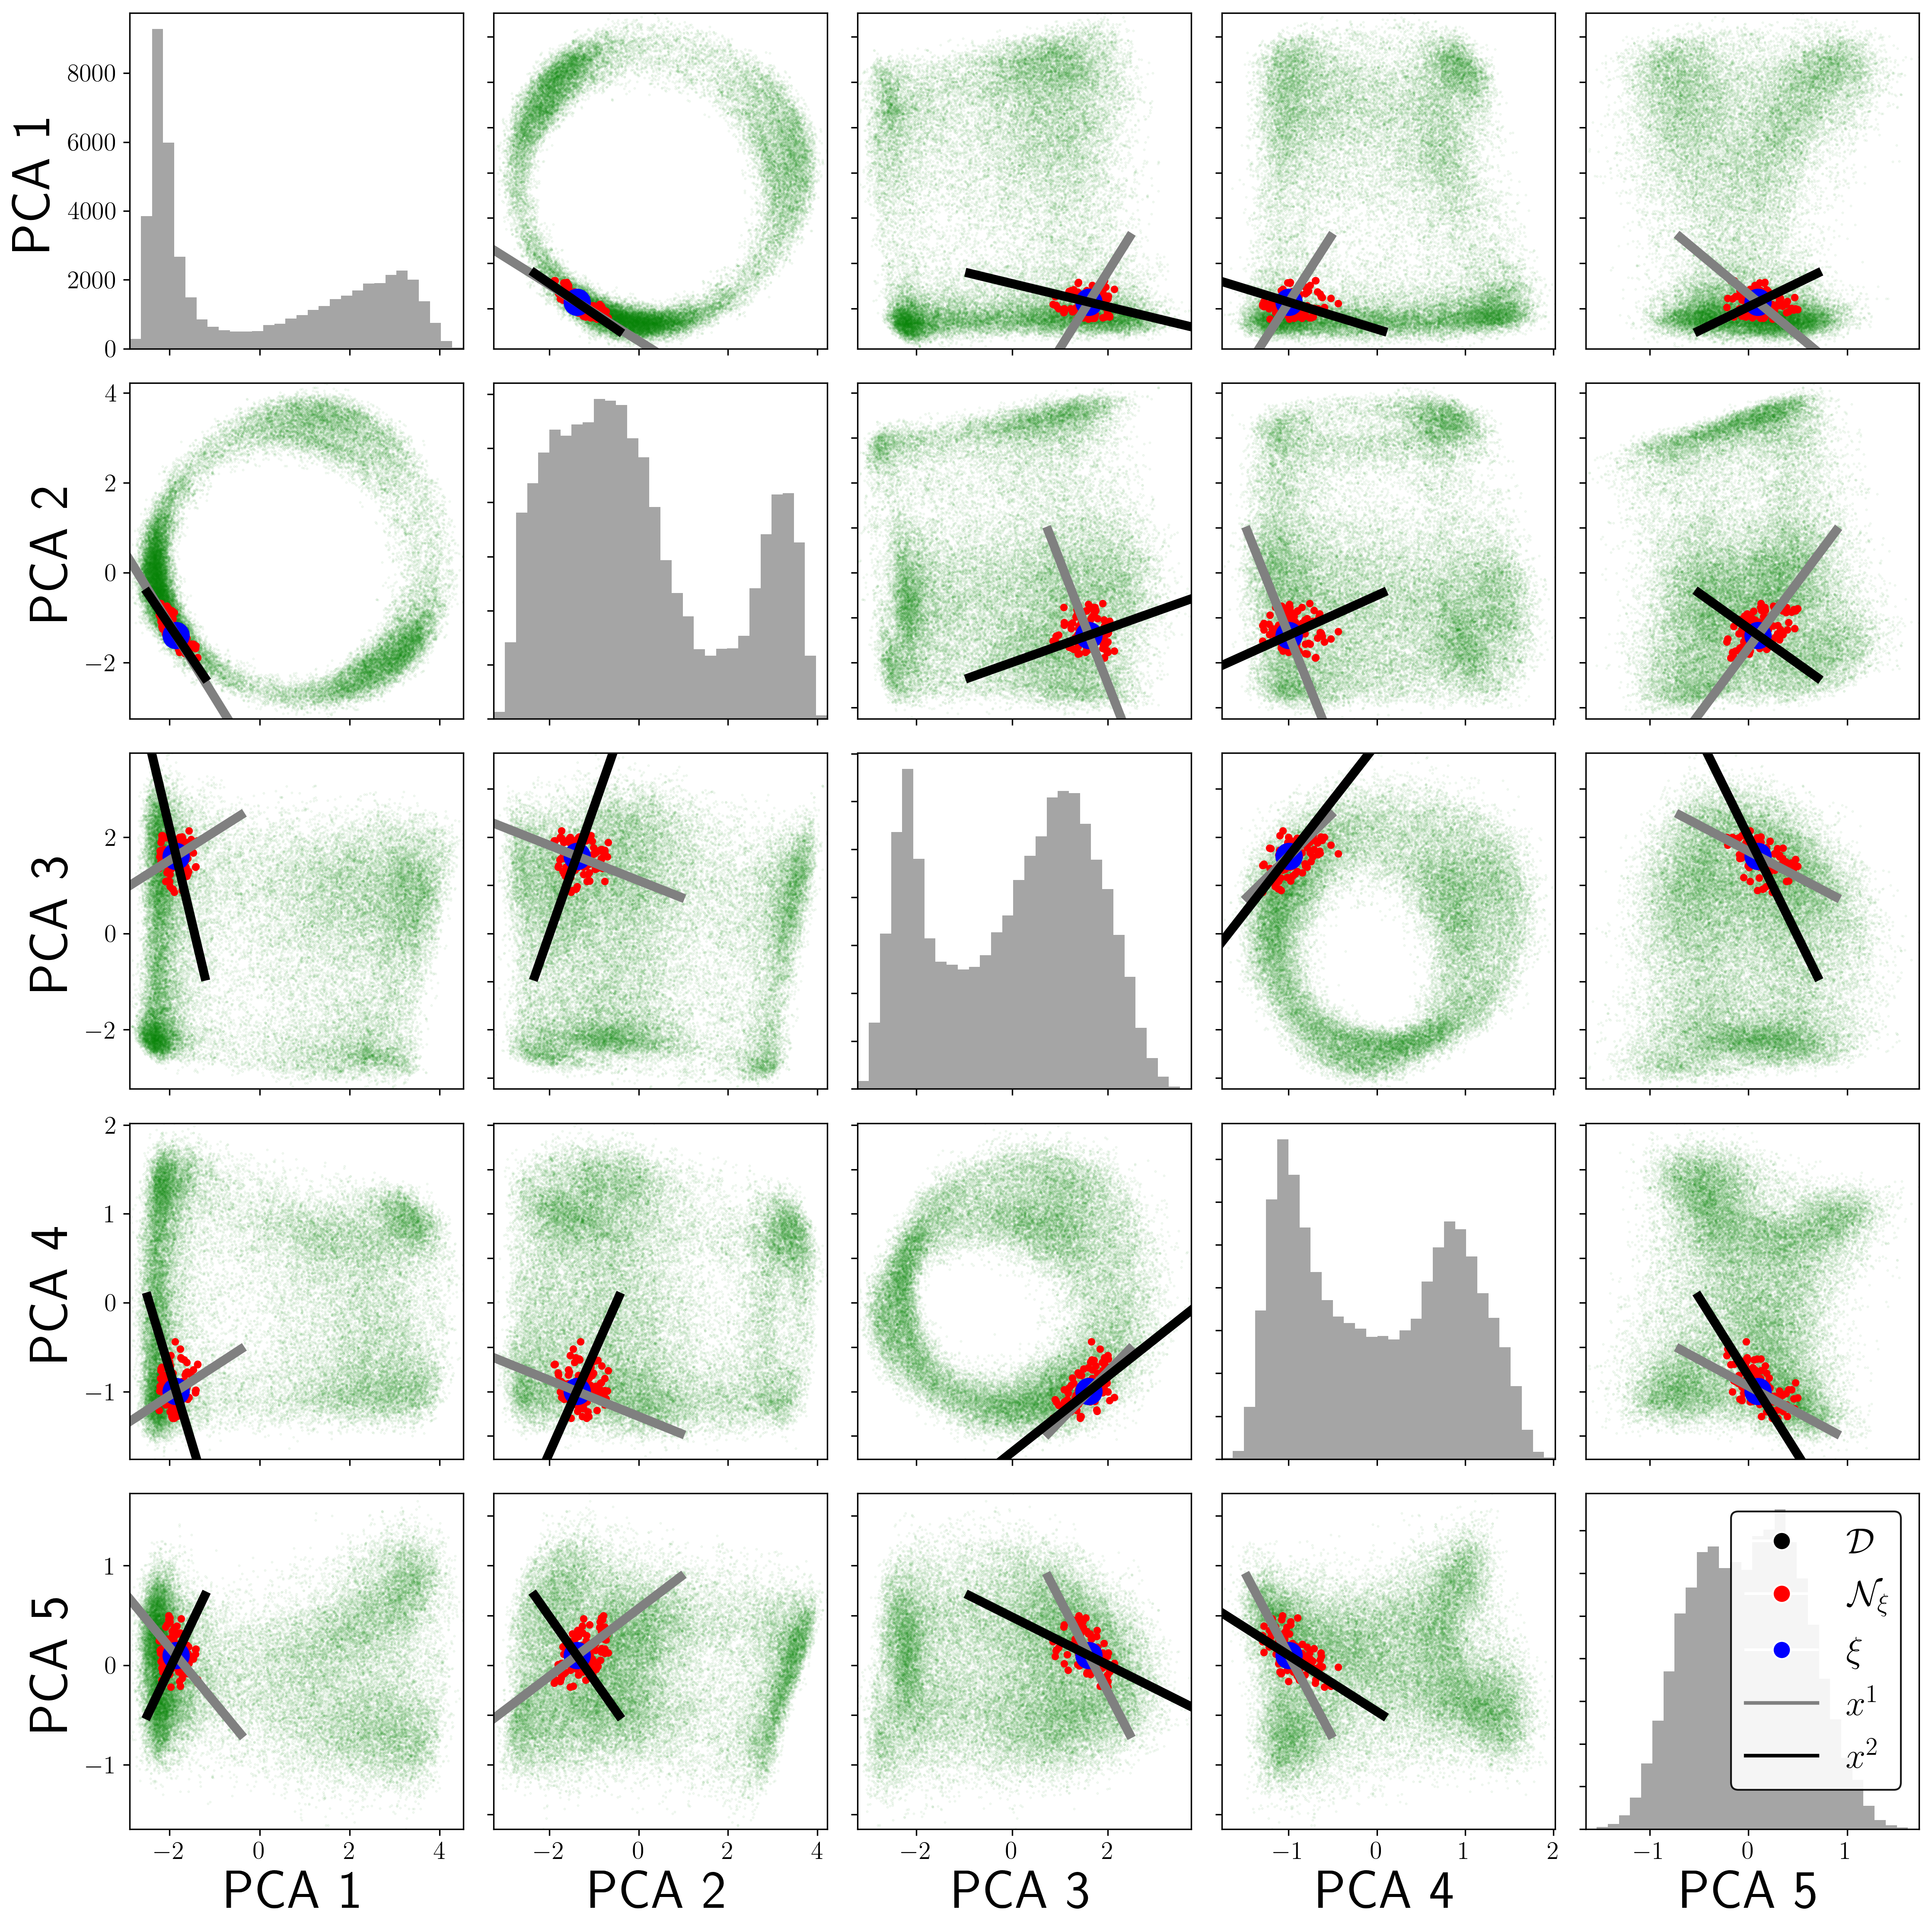
\includegraphics[width=2.5in]{img/tangentspaces.png}
    \caption*{A neighborhood and tangent space plotted in top global PCA coordinates}
\end{figure}
\end{column}
\end{columns}


\end{frame}

\begin{frame}{Gradients}
\begin{itemize}
    \item We can compute dihedral angle gradients with autograd
    \item We then project $d_{\mathcal M} g (n) = (T_{\mathcal M} (n))^T d g (n)$
\end{itemize}
\small
\begin{figure}[!htp]
    \centering
    \begin{tabular}{p{2.5cm}p{2.5cm}p{2.5cm}p{2.5cm}}
        \includegraphics[width=0.25\textwidth, trim={2cm 3cm 5cm 0cm}, clip]{img/ethanol_g0.png} &
        \includegraphics[width=0.25\textwidth, trim={2cm 3cm 5cm 0cm}, clip]{img/ethanol_g1.png} &
          \includegraphics[width=0.25\textwidth, trim={2cm 3cm 5cm 0cm}, clip]{img/ethanol_g2.png} &
          \includegraphics[width=0.25\textwidth, trim={2cm 3cm 5cm 0cm}, clip]{img/ethanol_g3.png}  \\
        \includegraphics[width=0.2\textwidth]{img/tangent_0.png} &
        \includegraphics[width=0.2\textwidth]{img/tangent_1.png} &
         \includegraphics[width=0.2\textwidth]{img/tangent_2.png}  &
          \includegraphics[width=0.2\textwidth]{img/tangent_3.png} 
    \end{tabular}
    %\vspace{-2cm}
    \caption*{ Gradients $dg^p = \frac{\partial g^p }{\partial x^d} $ of four dihedral angles $g^p:\mathcal M \to \mathbb R$ with respect to coordinates $x^1 \dots x^D$ of tangent space $\mathcal {T}_{\mathcal M} (n)$}
\end{figure}
\end{frame}


\begin{frame}{Normalization}
\begin{itemize}
    \item We normalize $d g^p(n)= \frac{\sqrt{N} d g^p(n)}{  \|d g^p([N])\|_F}$ prior to projection to favor gradient fields which are more tangent to the manifold
\end{itemize}
\begin{figure}[!htp]
    \centering
    \begin{tabular}{ccc}
        \includegraphics[width=0.3\textwidth, trim={3cm 2cm 5cm 3cm}, clip]{img/raw.png} &
        \includegraphics[width=0.3\textwidth, trim={3cm 2cm 5cm 3cm}, clip]{img/norm.png} &
          \includegraphics[width=0.3\textwidth, trim={3cm 2cm 5cm 3cm}, clip]{img/proj.png}  \\
           \centering
        $dg$ &
         \centering
       $dg$ (normalized) &
        \centering
        $d_{\mathcal M} g$
    \end{tabular}
    \caption*{Gradients of example functions \textcolor{red}{$g^1$} and \textcolor{blue}{$g^2$} for $B = 2, D = 1$}
\end{figure}
\begin{itemize}
    \item Note: gradients of dihedral angles w.r.t. planar angles are not well-defined and so we use $dg = d_{\mathbb R^{3N_a}} g (d_{\mathbb R^{3N_a}} \alpha)^{\dagger_{3N_a - 7}}$
\end{itemize}
\end{frame}

\begin{frame}{Results}
\begin{figure}[!htp]
    \centering
    \begin{tabular}{p{3cm}p{3cm}p{3cm}}
        \includegraphics[width=0.2\textwidth]{img/reg_small.png} &
        \includegraphics[width=0.35\textwidth, trim={3cm 0cm 0cm 4cm}, clip]{img/ethanol_g0.png} &
          \includegraphics[width=0.35\textwidth, trim={3cm 0cm 0cm 4cm}, clip]{img/ethanol_g2.png}  \\
        \includegraphics[width=0.2\textwidth, trim={0cm 0cm 3cm 0cm}, clip]{img/cosines_sellasso_small.png} &
        \includegraphics[width=0.35\textwidth, trim={3cm 0cm 0cm 3cm}, clip]{img/ethanol_small_embedding_0.png} &
          \includegraphics[width=0.35\textwidth, trim={3cm 0cm 0cm 3cm}, clip]{img/ethanol_small_embedding_1.png} 
    \end{tabular}
    %\vspace{-2cm}
    \caption*{Results for one replicate with $P=12$ dictionary functions implicitly defined by the ethanol bond diagram}
\end{figure}
\end{frame}
% 1 

\section{Experiments}
\label{sec:experiments}

% fix algorithm shortcuts, add greedy and brute to the supplement
We compare \tsip~ and \greedy~ on the Iris and Wine datasets \citep{misc_iris_53, misc_wine_109, scikit-learn}, as well as the Ethanol dataset from \citet{Chmiela2018-at, Koelle2022-ju}.
The latter is an interpretability dataset where a dictionary of interpretable features are evaluated for their ability to parameterize the data manifold through computation of their Jacoban matrices and projection onto estimated tangent spaces (see \citet{Koelle2022-ju} for preprocessing details).
Statistical replicas for Wine and Iris are created by resampling across $P$, while for Ethanol they are created by sampling from different points on the data manifold.
For basis pursuit, We use the SCS interior point solver \citep{ocpb:16} from CVXPY \citep{diamond2016cvxpy, agrawal2018rewriting}, which is able to push sparse values arbitrarily close to 0 \citep{cvxpy_sparse_solution}.

\begin{figure}[h]
\centering
\subcaptionbox{Boxplot of $\widehat S_{g}$. \label{fig:boxplot1}}
{\includegraphics[width=.3\textwidth]{/Users/samsonkoelle/convexlocalisometry/figures/Figure2b.png}}
\subcaptionbox{Boxplot of $\widehat S_{TS}$. \label{fig:boxplot2}}
{\includegraphics[width=.3\textwidth]{/Users/samsonkoelle/convexlocalisometry/figures/Figure2b.png}}
\subcaptionbox{Boxplot of $\widehat S_{third}$. \label{fig:boxplot3}}
{\includegraphics[width=.3\textwidth]{/Users/samsonkoelle/convexlocalisometry/figures/Figure2b.png}}
\caption{Comparison with isometry loss.}
\label{fig:boxplots}
\end{figure}

\begin{table}[h!]
\centering
\begin{tabular}{c|c|c|c|c|c|}
\hline
Name & $D$ & $P$ & $n$ & $I$ & $|\widehat{\mathcal{S}_1}|$ \\ \hline
% Add your data here
Iris & 1 & 2 & 3 & 4 & 5 \\ \hline
Wine & 6 & 7 & 8 & 9 & 10 \\ \hline
Ethanol & 11 & 12 & 13 & 14 & 15 \\ \hline
\end{tabular}
\caption{Experimental parameters and results.
For the Wine dataset, even \brute~ on $\widehat {\mathcal S}_1$ is prohibitive in $D=13$, and so we truncate our inputs to $D=5$.}
\label{tab:sample}
\end{table}
\section{Discussion}
\label{sec:discussion}

This extension is a local version of Tangent Space Lasso.
%The Hoeffding bound
%Dimension estimation, the failure of duality
%The presence of curvature

Tangent space basis pursuit satisfies a similar property \cite{Koelle2022-lp} but the normalization process differs.

It could be used in the stiching step of an algorithm like the kohli one
We leave aside the question of patch alignment \cite{https://arxiv.org/pdf/2303.11620.pdf, LDLE paper}.
The full gradient approach.
In this case normalization prior to projection is subsumbmed by the larger coefficients needed to get the tangent space.
Good news is tangent space estimation need not be performed.
Let's compare the coefficients involved in projecting versus not projecting.
We can perform regression in the high dimensional space instead of projecting on span of target variable.

With respect to pseudoinverse estimation, sparse methods have been applied in \cite{Sun2012-vp}

Even though by Lagrangian duality, the basis pursuit solution corresponds to $\lambda$ approaching $0$, the solution is sparse \cite{Tropp04-ju}.
about the lasso is that all coefficients enter the regularization path.
As we see by the correspondence between $\lambda$ approaching $0$ and the basis pursuit problem, some coefficients in fact do not go to $0$. 


\bibliography{ref}

\section{Supplement}
% NOTE (Sam): make sure to add basis pursuit equivalence
We give proofs in support of the propositions in the main text and supplemental experimental information to better contextualize the results. 

\subsection{Proofs}
\label{sec:proofs}

\subsubsection{Proof of Proposition \ref{prop:basis_pursuit_selection_invariance}}
\label{proof:basis_pursuit_program_invariance}

In this proof we first show that the penalty $\|\beta\|_{1,2}$ is unchanged by unitary transformation of $\beta$.

 \begin{proposition}{Loss equivalence}
 \label{prop:basis_pursuit_loss_equivalence}
 Let $U \in \mathbb R^{D \times D}$ be unitary.
 Then $\|\beta\|_{1,2} = \|\beta U \|$.
\end{proposition}

\begin{proof}
\begin{align}
\|\beta U \|_{1,2} &= \sum_{p = 1}^P \| \beta_{p.} U \| \\
&= \sum_{p = 1}^P \| \beta_{p.} \| \\
&= \|\beta \|_{1,2}
\end{align}
\end{proof}

We then show that this implies that the resultant loss is unchanged by unitary transformation of $\mathcal X$.

\begin{proposition}
 \label{prop:basis_pursuit_loss_equivalence}
 Let $U \in \mathbb R^{D \times D}$ be unitary.
 Then $\widehat \beta  (U \mathcal X) = \widehat \beta  ( \mathcal X) U$.
\end{proposition}

\begin{proof}
\begin{align}
\widehat \beta  (U \mathcal X)  &= \arg \min_{\beta \in \mathbb R^{P \times D}} \|\beta\|_{1,2}  \; : \; I_{D} = U X \beta \\
&= \arg \min_{\beta \in \mathbb R^{P \times D}} \|\beta\|_{1,2}  \; : \; U^{-1} U = U^{-1} U X \beta U \\
&= \arg \min_{\beta \in \mathbb R^{P \times D}} \|\beta\|_{1,2}  \; : \;  I_D = X \beta U \\
&= \arg \min_{\beta \in \mathbb R^{P \times D}} \|\beta U \|_{1,2}  \; : \;  I_D = X \beta U \\
&= \arg \min_{\beta \in \mathbb R^{P \times D}} \|\beta \|_{1,2}  \; : \;  I_D = X \beta.
\end{align}
\end{proof}

\subsubsection{Proof of Proposition \ref{prop:unitary_selection}}
\label{sec:local_isometry_proof}

In support of the proposition in the main text, we give a more general theorem which illustrates the key features of the method.
From there, it is a straightforward step to specify to the chosen normalization.

 \begin{proposition}[Generalized unitary selection]
\label{prop:generalized_unitary_selection}
Given a matrix $\mathcal X \in \mathbb R^{D \times P}$ with a rank $D$ submatrix $\mathcal X_{.\mathcal S} \in \mathbb R^{D \times D}$ that is the unique $D \times D$ rank $D$-unitary submatrix, and let $n_q$ be a normalization composed of normalizing functions $q$ that satisfy the conditions of Definition \ref{def:symmetric_normalization}, then  $\mathcal S = S(\widehat{\beta}_{q}^P (\mathcal X)))$.
 \end{proposition}
 
 \begin{proof}

This proof consists of showing that $D$ is the theoretical lower limit for the loss.
This value is clearly obtained by $\beta_{S.}$ unitary and $\beta_{S^C.}$ zero elsewhere, so the real work consists of showing that solutions with $\|\beta\|_{1,2} < D$ are not possible, and that solutions with $\|\beta\|_{1,2}  = D$ are only obtained by $D$ sparse solutions.

% NOTE (Sam): I think this should just be the main proposition.
\begin{proposition}[Unitary Preference]
% Given $X$ as in Proposition \ref{prop:generalized_unitary_selection}, let $\beta = \widehat \beta^P_q(X)$.  Then $\|\beta^*\|_{1,2} = D$.
Given $X$, $\|\beta(X)\|_{1,2} \geq D$ and $\|\beta(X)\|_{1,2} = D \implies X_{.S(\beta)}$ is unitary. 
% NOTE (Sam): need to differentiate unitary and semi-unitary?
\end{proposition}

\begin{proof}

This proof proceeds by showing that replacing $X_{.S(\beta)}$ with a unitary matrix - without loss of generality $I_D$ - leads to the existence of a solution $\beta_S' = X_S \beta_S$ such that $\|\beta_S\|_{1,2} \geq \|\beta_S' \|_{1,2}$.


We want to show that 
\begin{align}
\| X_{.S} \beta_{S.}  \|_{1,2} \leq \|\beta_{S.}\|_{1,2} % this may not be true.  it can cause a sparse solution to become non sparse.
\end{align}
We rewrite 
\begin{align}
\| X_{.S} \beta_{S.}  \|_{1,2}  &= \sum_{d=1}^D \| X_{dS}  \beta_{S.}  \|_{2}  
\end{align}
and
\begin{align}
\| \beta_{S.}  \|_{1,2}  &= \sum_{p \in S} \| \beta_{S.}  \|_{2}.
\end{align}
%We know that $\| X_{.p} \|_2 \leq 1.$


We then show that replacing the output of vectors not in $S$ lowers loss as well.



%By the conditions in Definition  \ref{def:symmetric_normalization}, the maximum length for vectors $\mathcal X^q_{.p}$ is attained when $\|\mathcal X_{.p}\|_2 = 1$.
%By Proposition \ref{prop:unitary_basis}, this is the case for unitary matrices, but it is also true for matrices for which $\mathcal X^q_{.p}$ are not orthogonal.

The next component of the argument deals with elements of $[P]$ which are not contained within $\mathcal S$.
We show that zeroing components of $\beta_{p.}'$ where $p \not \in S$ and compensating for the removal by altering the loadings within $\mathcal S$ results in lower loss.

% NOTE (Sam): need to clarify that \beta_{c.} is a vector
% NOTE (Sam): beta_c is not ' since its only operated on by the change from the earlier theorem.  Refitting would lead to a changed value.

\begin{proposition}[Support replacement]
\begin{align}
\|\beta_{S}'\|_{1,2} + \|\beta_{S^C}\|_{1,2} \geq D
\end{align}
\end{proposition}
\end{proof}

\end{proof}
\subsubsection{Proof of Proposition \ref{prop:lasso_selection_equivalence} }

This proof proceeds similarly to the proof of Proposition  \ref{prop:basis_pursuit_selection_equivalence} .
Proposition \ref{prop:lasso_selection_equivalence} relies on the fact that its loss is invariant under any unitary transformation.
As a corollary, this fact gives that the identify matrix which is the "dependent variable" in the regression equation may be replaced by any $d \times d$ unitary matrix.
For Proposition \ref{prop:basis_pursuit_selection_equivalence}, the loss is also invariant under unitary, transformation, but we also check that this transformation.
Once again, this also implies that any unitary matrix may replace the identity in the constraint.
%Minimizer?

 \begin{proposition}{Loss equivalence}
 \label{prop:lasso_loss_equivalence}
 Let $U \in \mathbb R^{D \times D}$ be unitary.
 Then $l_\lambda (\mathcal X, \beta) = l_\lambda (U \mathcal X, \beta U)$.
\end{proposition}

\begin{proof}
We can write 
\begin{eqnarray}
l^*(X^i) = l(\beta^i) = \sum_{j = 1}^p (\sum_{i'=2}^n \| \beta_{i'j.} \|_2^2 +  \|  \beta_{1j.}^i \|_2^2 )^{1/2}=  \sum_{j = 1}^p (\sum_{i'=1}^n \| \beta_{i'j.} U \|_2^2)^{1/2} = l^*(X)
\end{eqnarray}
where the second to last equality is because the norm $\|v\|_2^2 $ is unitary invariant.

\end{proof}

\begin{proposition}{Programmatic equivalence}
\label{prop:lasso_program_equivalence}
 Let $U \in \mathbb R^{D \times D}$ be unitary.
 Then $\hat \beta_{\lambda}  (U \mathcal X) = U\hat \beta_{\lambda} (\mathcal X)$.
\end{proposition}



\subsection{Experiments}




\end{document}